\documentclass[a4paper,12pt]{article}
% if you need additional LaTeX packages, add them here
\usepackage[margin=1in]{geometry}
\usepackage{graphicx, wrapfig, enumitem}
\usepackage{subcaption}
\usepackage{xcolor}
\usepackage{listings, ulem}
\usepackage[most]{tcolorbox}
\usepackage{multirow, multicol, tabularx, booktabs}
\usepackage{fancyhdr}
\usepackage{tikz}
\usepackage{hyperref}
\usepackage[simplified]{pgf-umlcd}
\usepackage{subfiles}
\usepackage[linguistics]{forest}
\usepackage{caption}
\usepackage{circuitikz}
\usepackage{tcolorbox}
\usepackage{courier}

\graphicspath{{Resources/}}


\setlist{nolistsep}
\setlength{\parindent}{0in}


\usetikzlibrary{decorations.markings}
\usetikzlibrary{calc}
\tikzset{middlearrow/.style={
        decoration={markings,
            mark= at position 0.5 with {\arrow{#1}} ,
        },
        postaction={decorate}
    }
}
\def\centerarc[#1](#2)(#3:#4:#5)% Syntax: [draw options] (center) (initial angle:final angle:radius)
    { \draw[#1] ($(#2)+({#5*cos(#3)},{#5*sin(#3)})$) arc (#3:#4:#5); }



\hypersetup{colorlinks=true, linkcolor=blue!50!red, urlcolor=green!70!black}

% defining a warning box
\definecolor{orang}{RGB}{255,155,0}

\newtcolorbox[auto counter,number within=section]{warningbox}[1][]{
  enhanced jigsaw,colback=white,colframe=orang,coltitle=orang,
  fonttitle=\bfseries\sffamily,
  sharp corners,
  detach title,
  leftrule=22mm,
  % What you need %%%%%%%%%%%%
  underlay unbroken and first={\node[below,text=black,anchor=east]
  at ([xshift=-22.5pt]interior.base west) {\Huge  \textbf{!}};},
  %%%%%%%%%%%%%%%%%%%%%%%%
  breakable,pad at break=1mm,
  #1,
  code={\ifdefempty{\tcbtitletext}{}{\tcbset{before upper={\tcbtitle\par\medskip}}}},
}

\newenvironment{centerdiagram}[1][\topsep]
  {\setlength{\topsep}{#1}\par\kern\topsep\centering}% \begin{mycenter}[<len>]
  {\par\kern\topsep}% \end{mycenter}

\pagestyle{fancy}
\fancyfoot[L,C,R]{}
\fancyhead[L,C,R]{}
\fancyfoot[L]{}
% \fancyfoot[R]{\thepage}
\fancyhead[R]{TinyBot : \thepage}
\fancyhead[L]{
    \includegraphics[height=1cm]{CRoCLogo(mediumquality).png}
    % \includegraphics{Resources/CRoCLogo(mediumquality).png}
}


%%% Define Custom IDE Colors %%%
\definecolor{arduinoGreen}    {rgb} {0.17, 0.43, 0.01}
\definecolor{arduinoGrey}     {rgb} {0.47, 0.47, 0.33}
\definecolor{arduinoOrange}   {rgb} {0.8 , 0.4 , 0   }
\definecolor{arduinoBlue}     {rgb} {0.01, 0.61, 0.98}
\definecolor{arduinoDarkBlue} {rgb} {0.0 , 0.2 , 0.5 }

%%% Define Arduino Language %%%
\lstdefinelanguage{Arduino}{
  language=C++, % begin with default C++ settings 
%
%
  %%% Keyword Color Group 1 %%%  (called KEYWORD3 by arduino)
  keywordstyle=\color{arduinoGreen},   
  deletekeywords={  % remove all arduino keywords that might be in c++
                break, case, override, final, continue, default, do, else, for, 
                if, return, goto, switch, throw, try, while, setup, loop, export, 
                not, or, and, xor, include, define, elif, else, error, if, ifdef, 
                ifndef, pragma, warning,
                HIGH, LOW, INPUT, INPUT_PULLUP, OUTPUT, DEC, BIN, HEX, OCT, PI, 
                HALF_PI, TWO_PI, LSBFIRST, MSBFIRST, CHANGE, FALLING, RISING, 
                DEFAULT, EXTERNAL, INTERNAL, INTERNAL1V1, INTERNAL2V56, LED_BUILTIN, 
                LED_BUILTIN_RX, LED_BUILTIN_TX, DIGITAL_MESSAGE, FIRMATA_STRING, 
                ANALOG_MESSAGE, REPORT_DIGITAL, REPORT_ANALOG, SET_PIN_MODE, 
                SYSTEM_RESET, SYSEX_START, auto, int8_t, int16_t, int32_t, int64_t, 
                uint8_t, uint16_t, uint32_t, uint64_t, char16_t, char32_t, operator, 
                enum, delete, bool, boolean, byte, char, const, false, float, double, 
                null, NULL, int, long, new, private, protected, public, short, 
                signed, static, volatile, String, void, true, unsigned, word, array, 
                sizeof, dynamic_cast, typedef, const_cast, struct, static_cast, union, 
                friend, extern, class, reinterpret_cast, register, explicit, inline, 
                _Bool, complex, _Complex, _Imaginary, atomic_bool, atomic_char, 
                atomic_schar, atomic_uchar, atomic_short, atomic_ushort, atomic_int, 
                atomic_uint, atomic_long, atomic_ulong, atomic_llong, atomic_ullong, 
                virtual, PROGMEM,
                Serial, Serial1, Serial2, Serial3, SerialUSB, Keyboard, Mouse,
                abs, acos, asin, atan, atan2, ceil, constrain, cos, degrees, exp, 
                floor, log, map, max, min, radians, random, randomSeed, round, sin, 
                sq, sqrt, tan, pow, bitRead, bitWrite, bitSet, bitClear, bit, 
                highByte, lowByte, analogReference, analogRead, 
                analogReadResolution, analogWrite, analogWriteResolution, 
                attachInterrupt, detachInterrupt, digitalPinToInterrupt, delay, 
                delayMicroseconds, digitalWrite, digitalRead, interrupts, millis, 
                micros, noInterrupts, noTone, pinMode, pulseIn, pulseInLong, shiftIn, 
                shiftOut, tone, yield, Stream, begin, end, peek, read, print, 
                println, available, availableForWrite, flush, setTimeout, find, 
                findUntil, parseInt, parseFloat, readBytes, readBytesUntil, readString, 
                readStringUntil, trim, toUpperCase, toLowerCase, charAt, compareTo, 
                concat, endsWith, startsWith, equals, equalsIgnoreCase, getBytes, 
                indexOf, lastIndexOf, length, replace, setCharAt, substring, 
                toCharArray, toInt, press, release, releaseAll, accept, click, move, 
                isPressed, isAlphaNumeric, isAlpha, isAscii, isWhitespace, isControl, 
                isDigit, isGraph, isLowerCase, isPrintable, isPunct, isSpace, 
                isUpperCase, isHexadecimalDigit, 
                }, 
  morekeywords={   % add arduino structures to group 1
                break, case, override, final, continue, default, do, else, for, 
                if, return, goto, switch, throw, try, while, setup, loop, export, 
                not, or, and, xor, include, define, elif, else, error, if, ifdef, 
                ifndef, pragma, warning,
                }, 
% 
%
  %%% Keyword Color Group 2 %%%  (called LITERAL1 by arduino)
  keywordstyle=[2]\color{arduinoBlue},   
  keywords=[2]{   % add variables and dataTypes as 2nd group  
                HIGH, LOW, INPUT, INPUT_PULLUP, OUTPUT, DEC, BIN, HEX, OCT, PI, 
                HALF_PI, TWO_PI, LSBFIRST, MSBFIRST, CHANGE, FALLING, RISING, 
                DEFAULT, EXTERNAL, INTERNAL, INTERNAL1V1, INTERNAL2V56, LED_BUILTIN, 
                LED_BUILTIN_RX, LED_BUILTIN_TX, DIGITAL_MESSAGE, FIRMATA_STRING, 
                ANALOG_MESSAGE, REPORT_DIGITAL, REPORT_ANALOG, SET_PIN_MODE, 
                SYSTEM_RESET, SYSEX_START, auto, int8_t, int16_t, int32_t, int64_t, 
                uint8_t, uint16_t, uint32_t, uint64_t, char16_t, char32_t, operator, 
                enum, delete, bool, boolean, byte, char, const, false, float, double, 
                null, NULL, int, long, new, private, protected, public, short, 
                signed, static, volatile, String, void, true, unsigned, word, array, 
                sizeof, dynamic_cast, typedef, const_cast, struct, static_cast, union, 
                friend, extern, class, reinterpret_cast, register, explicit, inline, 
                _Bool, complex, _Complex, _Imaginary, atomic_bool, atomic_char, 
                atomic_schar, atomic_uchar, atomic_short, atomic_ushort, atomic_int, 
                atomic_uint, atomic_long, atomic_ulong, atomic_llong, atomic_ullong, 
                virtual, PROGMEM,
                },  
% 
%
  %%% Keyword Color Group 3 %%%  (called KEYWORD1 by arduino)
  keywordstyle=[3]\bfseries\color{arduinoOrange},
  keywords=[3]{  % add built-in functions as a 3rd group
                Serial, Serial1, Serial2, Serial3, SerialUSB, Keyboard, Mouse,
                },      
%
%
  %%% Keyword Color Group 4 %%%  (called KEYWORD2 by arduino)
  keywordstyle=[4]\color{arduinoOrange},
  keywords=[4]{  % add more built-in functions as a 4th group
                abs, acos, asin, atan, atan2, ceil, constrain, cos, degrees, exp, 
                floor, log, map, max, min, radians, random, randomSeed, round, sin, 
                sq, sqrt, tan, pow, bitRead, bitWrite, bitSet, bitClear, bit, 
                highByte, lowByte, analogReference, analogRead, 
                analogReadResolution, analogWrite, analogWriteResolution, 
                attachInterrupt, detachInterrupt, digitalPinToInterrupt, delay, 
                delayMicroseconds, digitalWrite, digitalRead, interrupts, millis, 
                micros, noInterrupts, noTone, pinMode, pulseIn, pulseInLong, shiftIn, 
                shiftOut, tone, yield, Stream, begin, end, peek, read, print, 
                println, available, availableForWrite, flush, setTimeout, find, 
                findUntil, parseInt, parseFloat, readBytes, readBytesUntil, readString, 
                readStringUntil, trim, toUpperCase, toLowerCase, charAt, compareTo, 
                concat, endsWith, startsWith, equals, equalsIgnoreCase, getBytes, 
                indexOf, lastIndexOf, length, replace, setCharAt, substring, 
                toCharArray, toInt, press, release, releaseAll, accept, click, move, 
                isPressed, isAlphaNumeric, isAlpha, isAscii, isWhitespace, isControl, 
                isDigit, isGraph, isLowerCase, isPrintable, isPunct, isSpace, 
                isUpperCase, isHexadecimalDigit, 
                },      
%
%
  %%% Set Other Colors %%%
  stringstyle=\color{arduinoDarkBlue},    
  commentstyle=\color{arduinoGrey},    
%          
%   
  %%%% Line Numbering %%%%
  numbers=left,                    
  numbersep=5pt,                   
  numberstyle=\color{arduinoGrey},    
  %stepnumber=2,                      % show every 2 line numbers
%
%
  %%%% Code Box Style %%%%
  breaklines=true,                    % wordwrapping
  tabsize=2,         
  basicstyle=\ttfamily\small
}

\lstset{language=Arduino}

\title{	
    \begin{center}
        \includegraphics[width=0.15\textwidth]{CRoCLogo(mediumquality).png}
    \end{center}
	\normalfont\normalsize
	\textsc{Curtin Robotics Club}\\ % Your university, school and/or department name(s)
	\vspace{25pt} % Whitespace
	\rule{\linewidth}{0.5pt}\\ % Thin top horizontal rule
	\vspace{20pt} % Whitespace
    {\huge TinyBot }\\
    % {\huge Assignment Report}\\ % The assignment title
	\vspace{12pt} % Whitespace
	\rule{\linewidth}{2pt}\\ % Thick bottom horizontal rule
	\vspace{12pt} % Whitespace
}

\author{\LARGE Ilke Dincer \\ \small ilke@curtinrobotics.org} % Your name

\date{\normalsize\today} % Today's date (\today) or a custom date

\begin{document}

\pagenumbering{gobble}
\maketitle

\pagebreak
\pagenumbering{roman}
\tableofcontents

\pagebreak
\pagenumbering{arabic}

\section{Introduction}

There are many different components of a robot; the most important being the microcontroller (the brain), the motors (the legs), and any sensors (how the robot sees the world).

This guide will take you through building a simple robot dubbed TinyBot. It has 2 wheels, a caster wheel, a battery, an arduino, and a breadboard.

\section{Assumed Knowledge}

The below knowledge is assumed for this project. Feel free to ask other CRoC members for help or explanation of the below concepts.


\begin{itemize}
    \item Basic circuit knowledge
    \begin{itemize}
        \item Current, Voltage, Resistance
        \item Series and Parallel
    \end{itemize}
    \item Breadboards
\end{itemize}

\section{Components}\label{sec:components}
 
\begin{tabularx}{\linewidth}{cccX}
    \toprule
    Component & Quantity & Price & Sources \\ \midrule
    Arduino Uno & 1 & \$5-\$80 & Arduino's are discussed in Section \ref{sec:microcontroller}. A genuine Arduino will cost about \$80, however Arduino clones can be bought online for as little as \$5. Ebay is a good starting point for finding an Uno. \\
    Breadboard & 1 & & \\
    N20 Motor & 2 & & \\
    H-Bridge & 1 & & \\  
    Wheels & 2& \$0 & The wheels for this project are 3D printed, and are supplied by the club. \\
    Caster Wheel & 1 & ? & The caster wheel consists of 2 parts, a marble and it's 3D printed casing. The 3D print will be supplied by the club at no charge, however you must source your own marble.\\
    \bottomrule
\end{tabularx}

\bigskip

Additional sensors can be bought and integrated with TinyBot, however that is not covered in this project guide. 

\section{Construction} \label{sec:construction}

\pagebreak
\section{Microcontroller} \label{sec:microcontroller}
\begin{wrapfigure}[4]{r}{0.3\textwidth}
    \vspace{-1cm}
    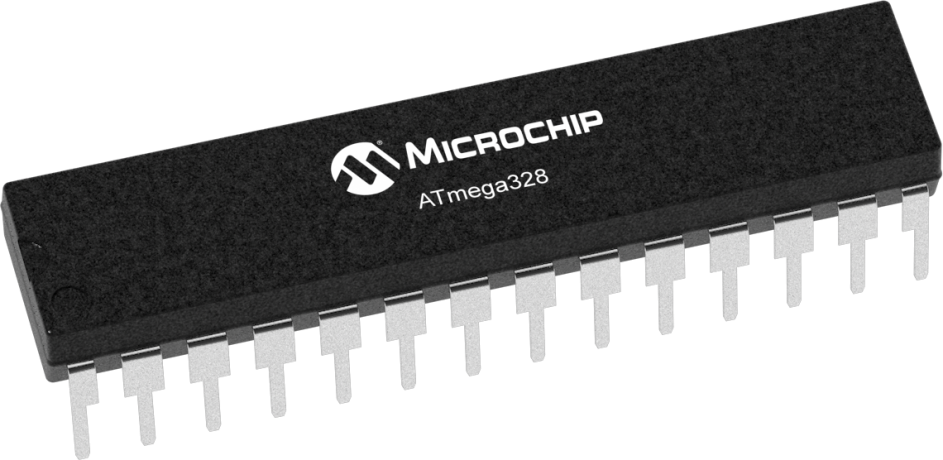
\includegraphics[width=0.25\textwidth]{medium-ATmega328-SPDIP-28.png}
    \captionof{figure}{A Microchip}
    \label{fig:microchip}
\end{wrapfigure}

A microcontroller is a really small microcomputer on a very small chip, see Figure \ref{fig:microchip}.
These are used in a variety of devices; including robots, vending machines, phones, computers, etc. \\

Arduino's are a development board; consisting of an microcontroller, power regulation, and input/output (also known as IO) pins. As microcontrollers are very tiny prototyping with them or using them to build something would be really difficult. The purpose of an arduino is to provide a medium that allows easy development with microcontrollers. There are many different kinds of arduinos, each using a different microchip. \\

\begin{wrapfigure}[10]{l}{0.35\textwidth}
    \centering
    \vspace{-0.5cm}
    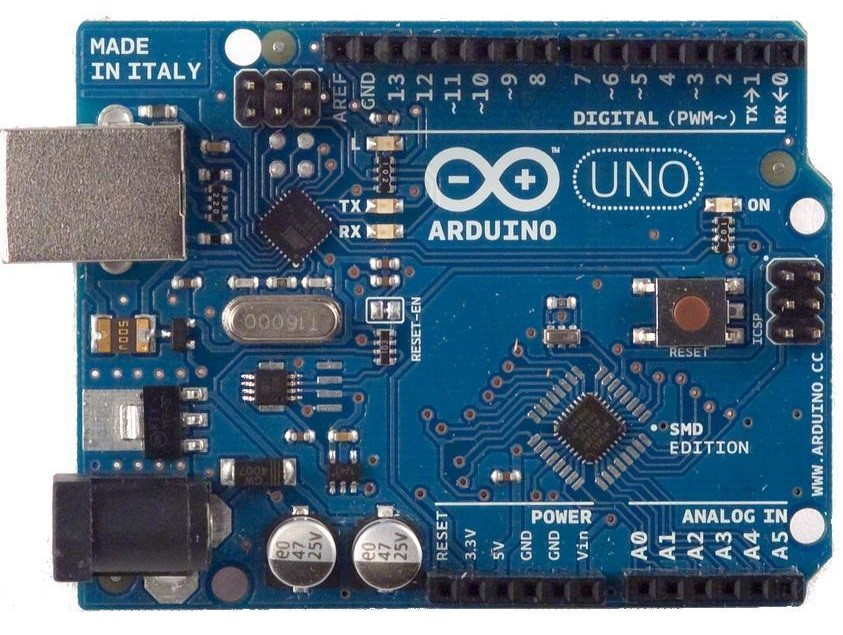
\includegraphics[width=0.33\textwidth]{arduino-uno.jpg}
    \caption{An Arduino Uno}
    \label{fig:arduino-real}
\end{wrapfigure}


% The Arduino used in this project is the Arduino Uno, which has an ATMega328p microchip as shown in Figure \ref{fig:microchip}. 
The difference between Arduino Uno, Mega, and Nano is the form factor and the microchip used on them. 
Figure \ref{fig:arduino-real} is what a real Arduino Uno looks like, though the colour and text may be different from brand to brand. Genuine Arduinos are quite expensive, there are many clones available which are much cheaper. Figure \ref{fig:arduino-pinout} shows a stylised view of an Uno, labelling all the different pinouts. \\

Arduino's and other development boards are used extensively by hobbyists, they are cheap, easy to use, and extremely versatile. Arduino's are used in nearly every CRoC project, and can be used in countless DIY projects. \\


An Uno has many different ports and pins. Figure \ref{fig:arduino-pinout} shows and labels all the different ports on a standard Uno. \\

An important distinction to make is between the pins 5V, 3.3V, and VIN. VIN stands for voltage in; and this port is used to supply power to the arduino from batteries. Power can also be supplied through the barrel jack connection, see the black rectangle like block on figure \ref{fig:arduino-pinout}. 

The 5V and 3.3V  pins supply 5 volts or 3.3 volts respectively for powering other commponents, such as LEDs, ICs, or sensors.  \\

\begin{warningbox}
    Never put supply voltage into the 3.3V or 5V pins; this will break the Arduino. 
\end{warningbox}


\begin{center}
    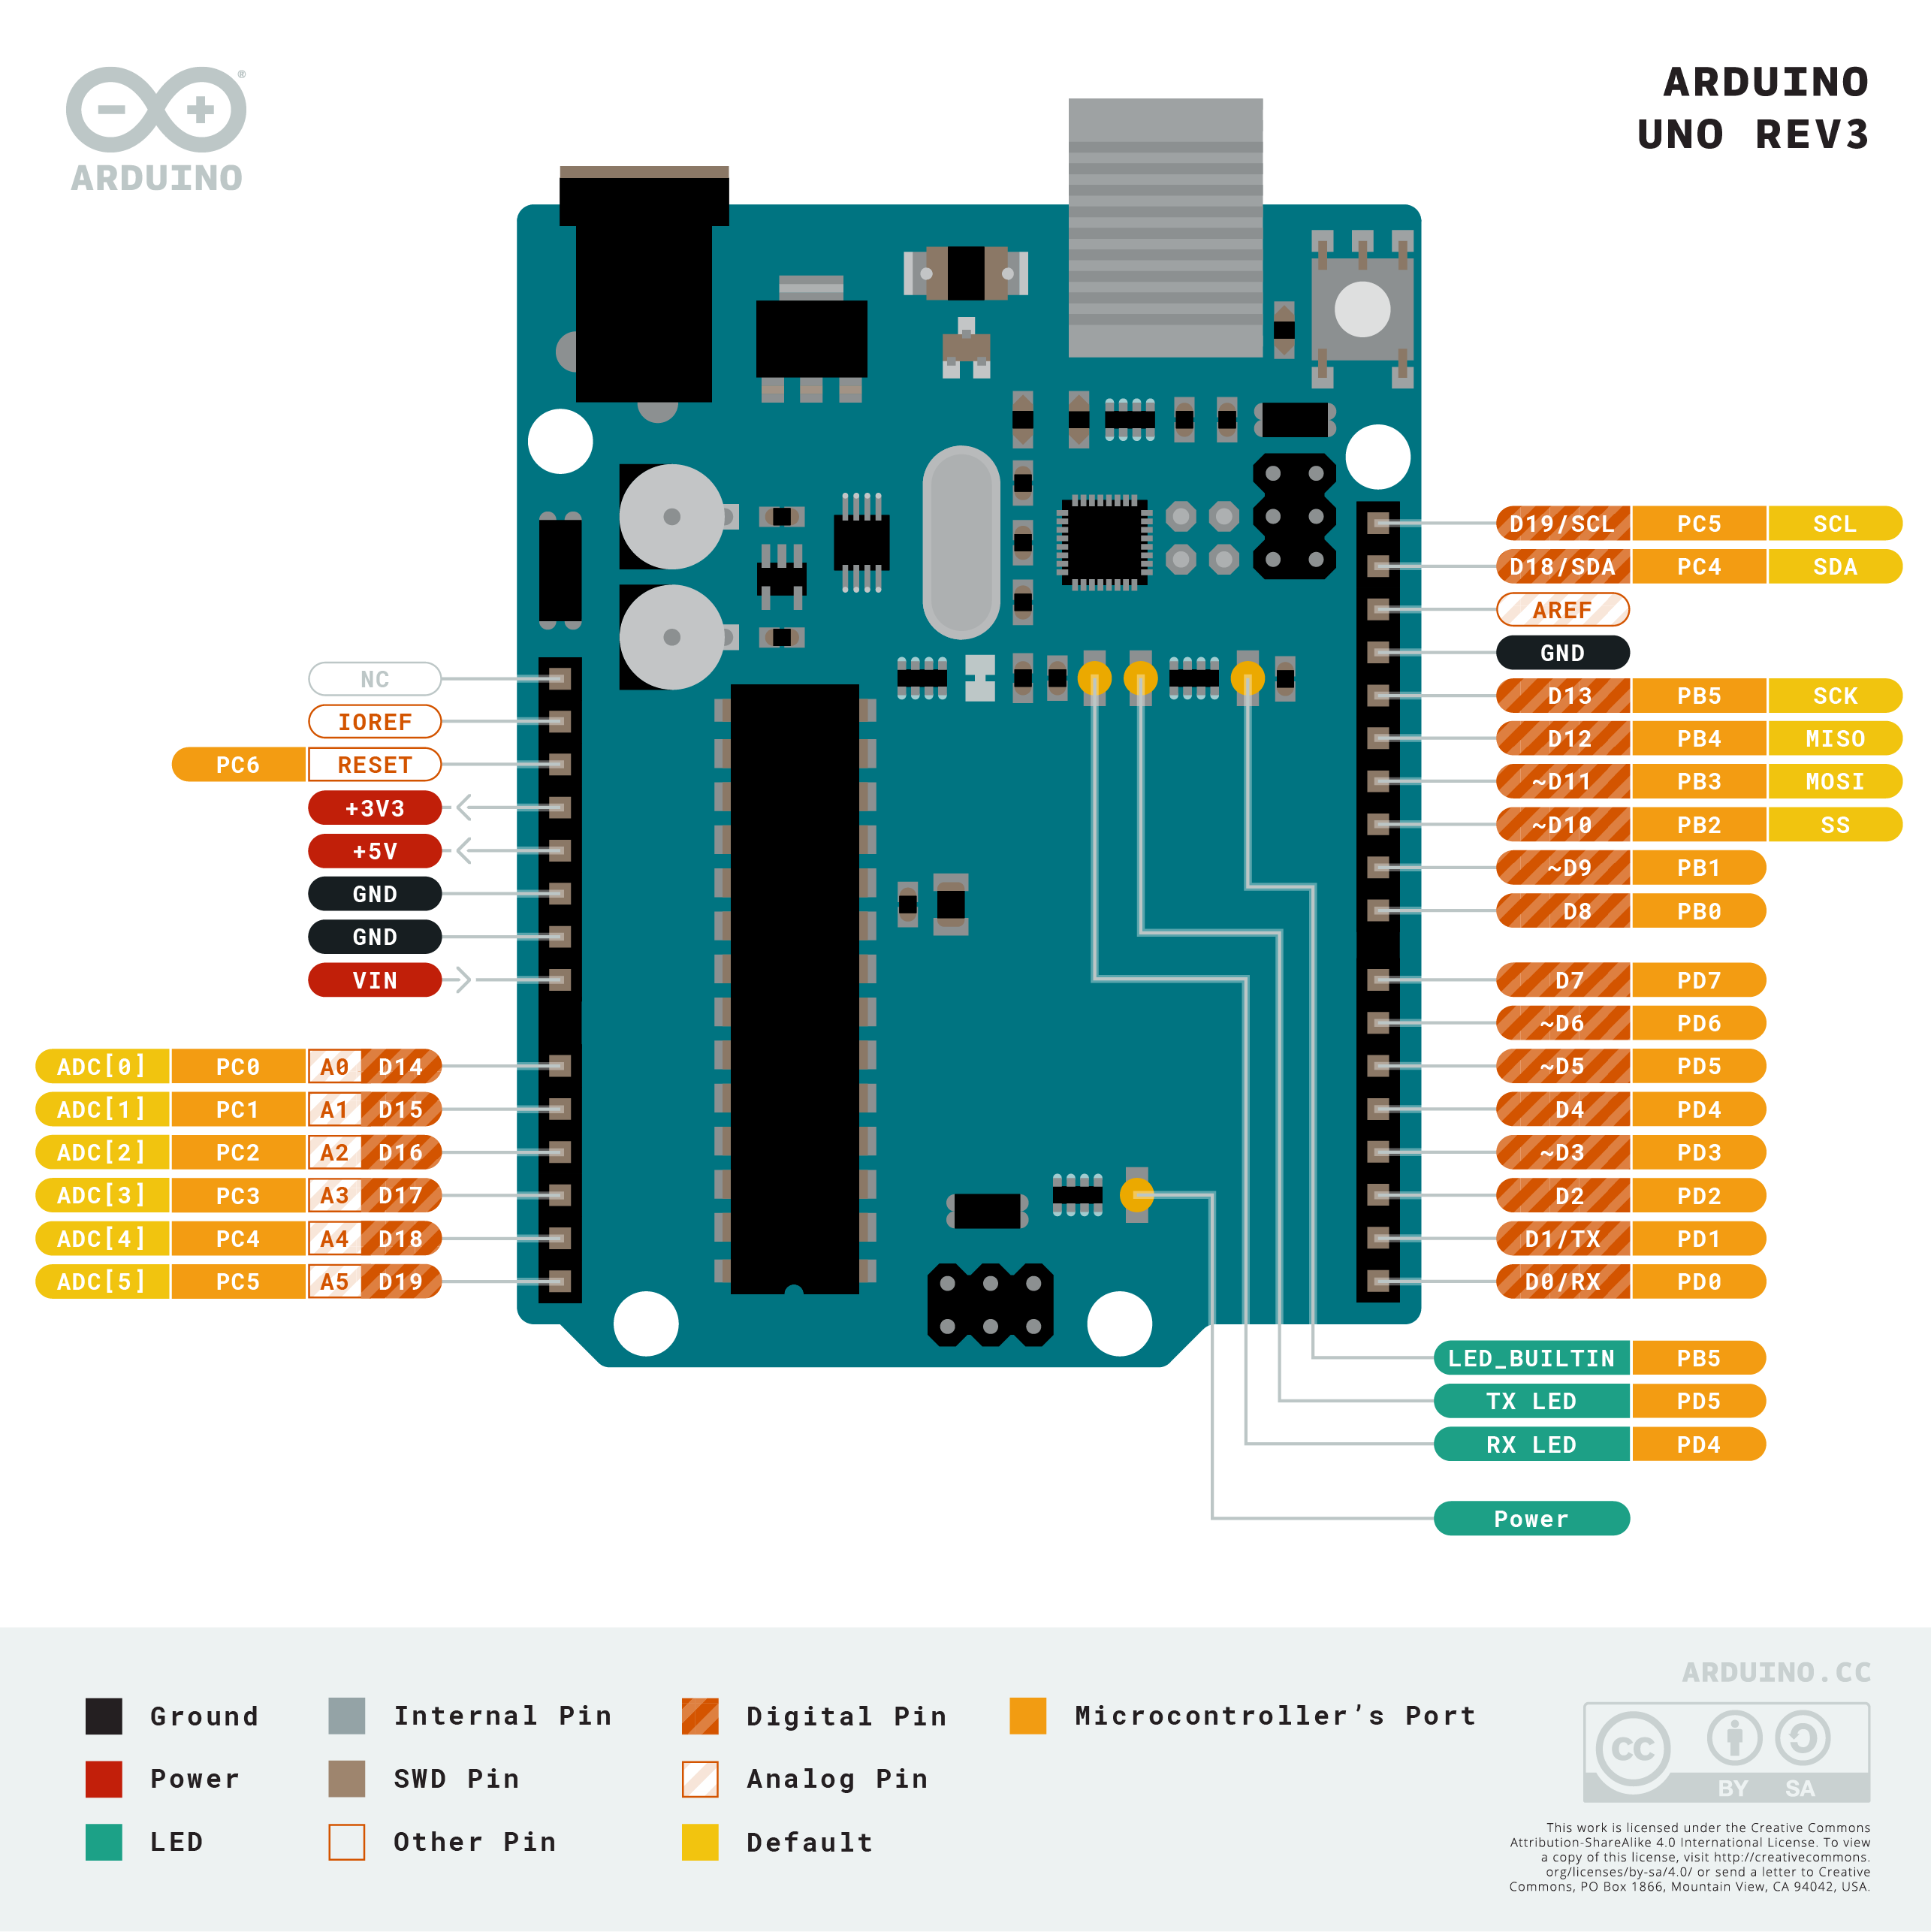
\includegraphics[width=\linewidth]{Pinout-UNOrev3_latest.png}
    \captionof{figure}{Pinout of Arduino Uno}
    \label{fig:arduino-pinout}
\end{center}


There are two different kinds of pins on an arduino, digital and analog. Look at the legend to see which pins are digital, The digital pin numbers all start with \lstinline[]!D!, just as the analog pins start with \lstinline[]!A!.
% (notice the pins on the right of the diagram labelled \lstinline[]!D0! to \lstinline[]!D13!) 
Analog pins can also be used as digital pins, but digital pins cannot be used as analog pins. \\


Digital pins can be set to \lstinline[]!HIGH! or \lstinline[]!LOW!, think of it like a button it can be on or off. Setting a pin to \lstinline[]!HIGH! turns it on, and \lstinline[]!LOW! turns it off. As circuits get more complicated, it is possible that setting a pin to \lstinline[]!LOW! will enable a part of the circuit; though for beginners it is best to think of \lstinline[]!HIGH! as on and \lstinline[]!LOW! as off; especially when working with a H-Bridge. 

% \$TODO - ANALOG PINS
\newpage
\section{Motor} \label{sec:motor}
gearbox, motor

To follow this guide it is not necessary to have an understanding of how motors work, though it may be interesting for you to learn. \href{https://www.explainthatstuff.com/electricmotors.html}{This} link has a good indepth explanation.


Motors turn in proportion to the amount of current put through them. More current means a faster motor. 

When a motor stalls, it stops rotating. This happens when there is more force acting on the motor shaft than the motor can overcome. The stall torque of a motor is the maximum current drawn when a motor stalls, in other words, applying its maximum torque. \\


Similarly, free current is the current drawn when the motor is rotating freely, under no load. 

\bigskip


Each motor has a certain amount of torque it can provide. Gearboxes can be attached to a motor to increase the amount of torque provided, and change the rotations per minute (RPM) of the motor. 


% $TODO - Someone who knows about gearboxes, please complete this section. 



\pagebreak
\section{Motor Controller} \label{sec:motorcontroller}

The motors used in this guide, the N20 motors, have a stall current of 1.6A (see section \ref{sec:motor} for what stall current means). The digital pins on an Arduino Uno supply at most 40mA. This is not enough to power the motors.\\ 

To get around this, the Arduino instead interfaces with a \textbf{motor controller}. Motor controllers have a seperate power supply that can supply enough current to drive the motor. Motor controllers also have digital inputs that allow control of the motor. \\


An added benefit of using a motor controller is that it is possible to control the direction and the speed of the motor. 

\bigskip

The phrase motor controller is often used as a generic term for any device, circuit, or IC which controls a motor. However, motor controllers are a circuit that consists of a motor driver, and some digital harness that acts as an interface to the driver. Motor controllers can be dropped into a circuit and easily controlled, allowing feedback from the motor and more control than a simple driver provides. \\


\subsection{Motor Driver}
A basic motor-\textbf{driver} is a H-bridge. The simplest H-bridge is shown in the below schematics, as well as an explanation of how using a H-bridge allows control over the motors direction. 

\begin{center}
    \begin{circuitikz}
    \draw (0,2) -- (0,0) to
        (0,0) to[nos, l^=$1$] (2,0) to
        (2,0) to [nos, l^=$2$] (4,0) to
        (4,0) -- (4,2) to
        (4,2) to[nos, l^=$3$] (2,2) to
        (2,2) to[nos, l^=$4$] (0,2);
    \draw (2,1) node[elmech](motor){M};
    \draw (motor.north) -- (2,2);
    \draw (motor.south) -- (2,0);
    \draw (0,1) -- (-1,1) node[vee]{};
    \draw (4,1) -- (5,1) node[ground]{};
    % \draw (2,0) to[sV, color=white, name=M] (2,2);
    % \mymotor{M}{90};
    % \draw[rotate=2] (0,2) \mymotor{M}{90} (2,2);
    \end{circuitikz}
    % \captionof{figure}{}
\end{center}

When switches $1$ and $3$ are closed, the current will flow through the motor making it turn anticlockwise.
% in the motor will flow in one direction. 

\begin{center}
    \begin{circuitikz}
        \draw (0,2) -- (0,0) to
            % (0,0) to[o-o, l_=$1$] (2,0) to
            (0,0) -- node[above, yshift=1.5mm]{1} (2,0) to
            (2,0) to [nos, l^=$2$] (4,0) to
            (4,0) -- (4,2) to
            % (4,2) to[l_=$3$] (2,2) to
            (4,2) -- node[below, yshift=-1.5mm]{3} (2,2) to
            (2,2) to[nos, l^=$4$] (0,2);
        \draw (motor.north) -- (2,2);
        \draw (motor.south) -- (2,0);
        \draw[color=red!100, thick] (0,1) -- (-1,1) node[vee]{};
        \draw[color=red!100, thick] (4,1) -- (5,1) node[ground]{};
     
        \begin{scope}[>=latex]
            \draw[->, color=red!100, thick] (-1,1) -- (0,1);
            \draw[->, color=red!100, thick] (0,1) -- (0,0);
            \draw[->, color=red!100, thick] (0,0) -- (2,0);
            \draw[->, color=red!100, thick] (2,0) -- (2,2);
            \draw[->, color=red!100, thick] (2,2) -- (4,2); 
            \draw[->, color=red!100, thick] (4,2) -- (4,1);
        \end{scope}
        \draw (2,1) node[elmech](motor){M};
        \centerarc[->](2,1)(-45:45:0.7);
        \centerarc[->](2,1)(135:225:0.7);
    \end{circuitikz}
\end{center}

In the same vein, closing switches 2 and 4 will cause the motor to turn clockwise. 
\begin{center}
    \begin{circuitikz}
        \draw (0,2) -- (0,0) to
            (0,0) to[nos, l^=$1$] (2,0) to
            % (2,0) to [nos, l_=$2$] (4,0) to
            (2,0) -- node[above, yshift=1.5mm]{2}(4,0) to 
            (4,0) -- (4,2) to
            (4,2) to[nos, l^=$3$] (2,2) to
            % (2,2) to[nos, l_=$4$] (0,2);
            (2,2) -- node[below, yshift=-1.5mm]{4} (0,2);
        \draw (motor.north) -- (2,2);
        \draw (motor.south) -- (2,0);
        \draw[color=red!100, thick] (0,1) -- (-1,1) node[vee]{};
        \draw[color=red!100, thick] (4,1) -- (5,1) node[ground]{};

        \begin{scope}[>=latex]
            \draw[->, color=red!100, thick] (-1,1) -- (0,1);
            \draw[->, color=red!100, thick] (0,1) -- (0,2);
            \draw[->, color=red!100, thick] (0,2) -- (2,2);
            \draw[->, color=red!100, thick] (2,2) -- (2,0);
            \draw[->, color=red!100, thick] (2,0) -- (4,0); 
            \draw[->, color=red!100, thick] (4,0) -- (4,1);
        \end{scope}
        \draw (2,1) node[elmech](motor){M};

        \centerarc[->](2,1)(45:-45:0.7);
        \centerarc[->](2,1)(225:135:0.7);

    \end{circuitikz}
\end{center}

If pins 4 \& 3 or pins 1 \& 2 are closed at the same time, a short circuit will be formed and the H-bridge will break. \\

\begin{minipage}{0.5\textwidth}\vspace{0pt}
    \begin{center}
        \begin{circuitikz}
            \draw (0,2) -- (0,0) to
                (0,0) to[nos, l^=$1$] (2,0) to
                (2,0) to [nos, l^=$2$] (4,0) to
                % (2,0) -- node[below, yshift=-1.5mm]{2}(4,0) to 
                (4,0) -- (4,2) to
                % (4,2) to[nos, l_=$3$] (2,2) to
                % (2,2) to[nos, l_=$4$] (0,2);
                (4,2) -- node[below, yshift=-1.5mm]{3} (2,2) to
                (2,2) -- node[below, yshift=-1.5mm]{4} (0,2);
            \draw (motor.north) -- (2,2);
            \draw (motor.south) -- (2,0);
            \draw[color=red!100, thick] (0,1) -- (-1,1) node[vee]{};
            \draw[color=red!100, thick] (4,1) -- (5,1) node[ground]{};
            
            \begin{scope}[>=latex]
                \draw[->, color=red!100, thick] (-1,1) -- (0,1);
                \draw[->, color=red!100, thick] (0,1) -- (0,2);
                \draw[->, color=red!100, thick] (0,2) -- (2.1,2);
                \draw[->, color=red!100, thick] (2,2) -- (4.01,2);
                % \draw[->, color=red!100, thick] (2,0) -- (4,0); 
                \draw[->, color=red!100, thick] (4,2) -- (4,1);
            \end{scope}
            \draw (2,1) node[elmech](motor){M};
    
        \end{circuitikz}
    \end{center}

\end{minipage}
\begin{minipage}{0.5\textwidth}\vspace{0pt}
    \begin{center}
        \begin{circuitikz}
            \draw (0,2) -- (0,0) to
                % (0,0) to[nos, l_=$1$] (2,0) to
                % (2,0) to [nos, l_=$2$] (4,0) to
                (0,0) -- node[above, yshift=1.5mm]{1}(2,0) to 
                (2,0) -- node[above, yshift=1.5mm]{2}(4,0) to 
                (4,0) -- (4,2) to
                (4,2) to[nos, l^=$3$] (2,2) to
                (2,2) to[nos, l^=$4$] (0,2);
                % (2,2) -- node[above, yshift=1.5mm]{4} (0,2);
            \draw (motor.north) -- (2,2);
            \draw (motor.south) -- (2,0);
            \draw[color=red!100, thick] (0,1) -- (-1,1) node[vee]{};
            \draw[color=red!100, thick] (4,1) -- (5,1) node[ground]{};    
    
            \begin{scope}[>=latex]
                \draw[->, color=red!100, thick] (-1,1) -- (0,1);
                \draw[->, color=red!100, thick] (0,1) -- (0,0);
                \draw[->, color=red!100, thick] (0,0) -- (2.1,0);
                % \draw[->, color=red!100, thick] (2,2) -- (2,0);
                \draw[->, color=red!100, thick] (2,0) -- (4,0); 
                \draw[->, color=red!100, thick] (4,0) -- (4,1);
            \end{scope}
            \draw (2,1) node[elmech](motor){M};
    
        \end{circuitikz}
    \end{center}
\end{minipage}

\bigskip \bigskip

Breaking a H-bridge is fairly common, especially the cheaper low power ones. Some higher end H-bridges are designed to prevent the H-bridge from shorting if the wrong pins are closed. 
Most motor-controllers will have this protection built-in, though most motor-drivers do not.


While working on this guide, don't worry if your H-bridge stops working suddenly, it is quite common to short them out. 

\bigskip


% In the case of the H-bridge, the voltage supplied (from the left on the diagrams displayed above) is a high enough voltage, with a high enough current, to drive the motor. The switches (1, 2, 3, 4) are, in their simplest form, a button that is closed upon a signal from the microcontroller. Switches require a very small amount of power to close, and so can be controlled directly from the motor controller. 


\subsection{Motor Controller}
% https://www.robotshop.com/en/roboclaw-2x30a-6-34vdc-regenerative-motor-controller.html


\begin{wrapfigure}[10]{l}{0.4\textwidth}
    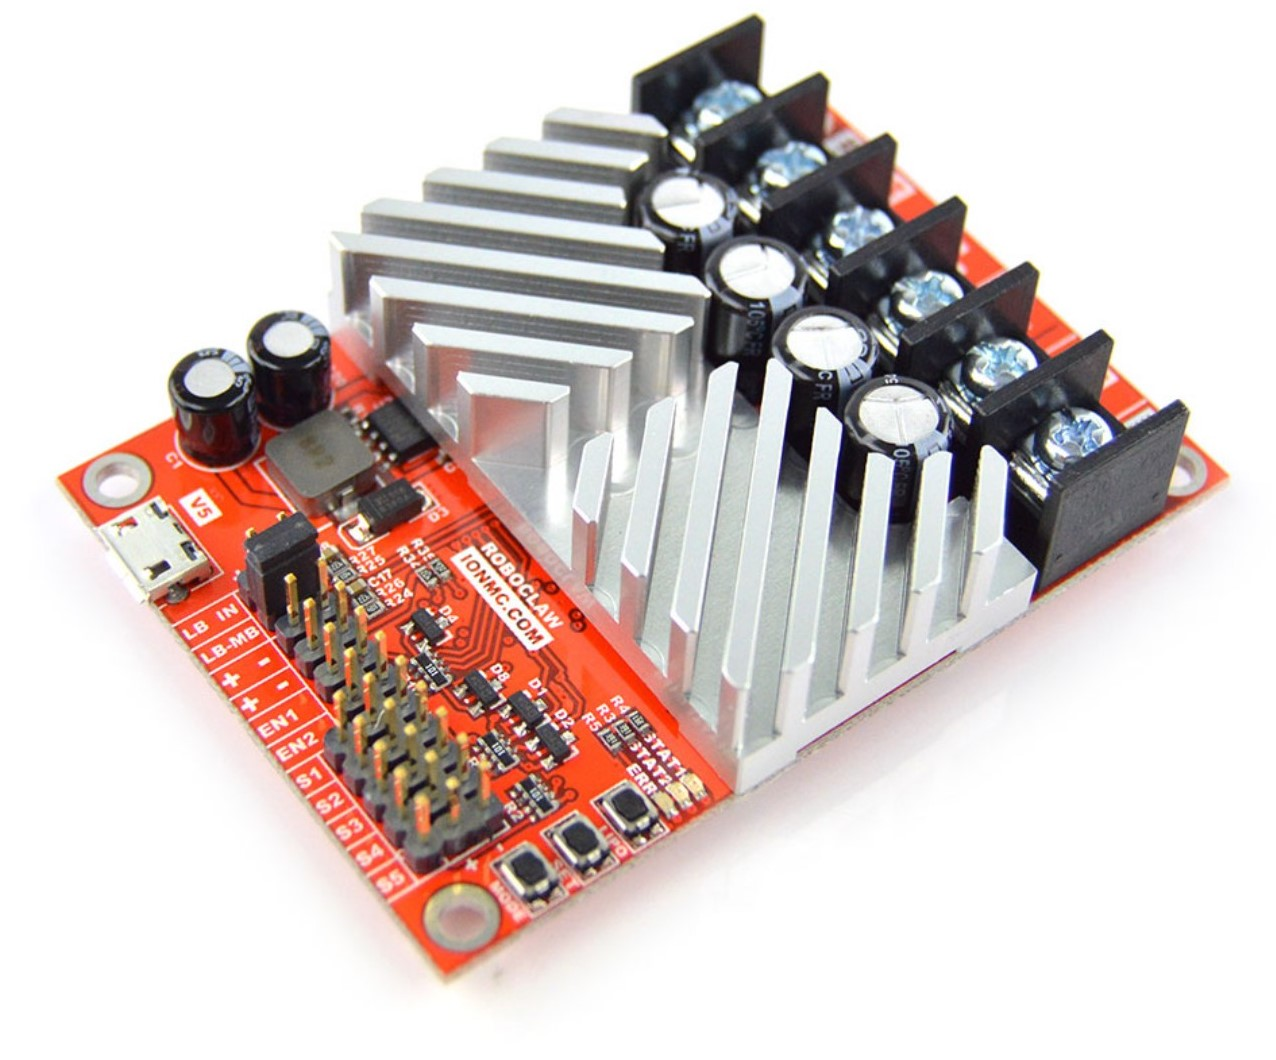
\includegraphics[width=0.4\textwidth]{roboclaw.jpg}
    \caption{\href{https://www.robotshop.com/media/files/content/b/bat/pdf/roboclaw_datasheet_2x30a-2.pdf}{RoboClaw Dual Channel DC Motor Controller}}
    \label{fig:roboclaw}
\end{wrapfigure}

A motor controller has a lot more features than a motor driver. See, for example, the RoboClaw (see Figure \ref{fig:roboclaw}) which has in built features such as PID tuning, data logging, diagnostic LEDs, and serial control. \\


The in-built control modes, as well as being capable of serial communication, is present only in motor controllers. Motor drivers are far simpler in comparision. \\


\bigskip \bigskip

\pagebreak
\section{Wiring} \label{wiring}
To wire up the circuit, get all the components listed in \ref{sec:components}.

Before starting construction on any project, it is always a good idea to wire up the circuit on a flat breadboard and arduino; as it is far easier to build the circuit on its own before putting together all the parts. \\


The H-bridge used in this project, 



Follow the wiring guide below.

\pagebreak
\section{Code}


To program an Arduino, you will need a USB cable, and a laptop/computer with the \href{https://www.arduino.cc/en/software}{Arduino IDE} installed. 



\begin{figure}[h]
    \centering
    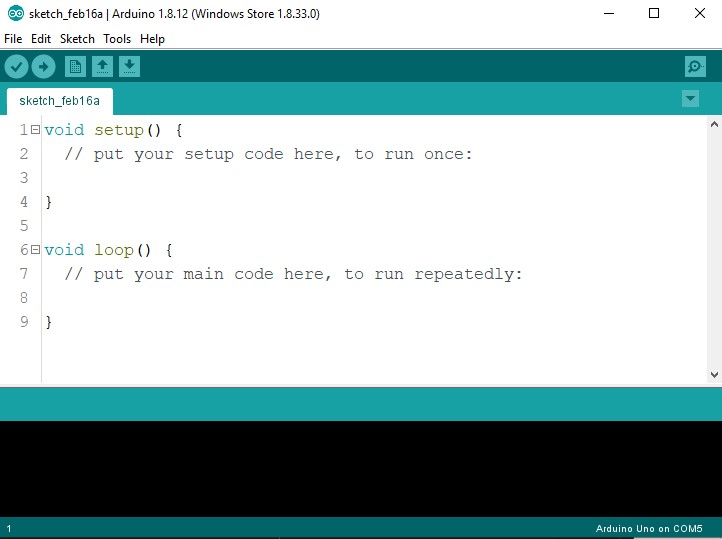
\includegraphics[width=0.7\textwidth]{arduino_ide.jpg}
    \caption{The Arduino IDE}
\end{figure}


Arduino's are programmed in the programming language /lstinline[]!C++!; though there are a few differences. The below code section details a few features of coding.


\begin{lstlisting}
// this is a comment

// variables declared not in a function will be accessible
// in all functions
int global_var = 0;

void setup {
  // everything in this function will run once
  // this code will run when the board is powered on, 
  // or when the reset button is pressed
}

void loop {
  // everything in this function will run repeatedly
}

\end{lstlisting}
\bigskip

\pagebreak
A useful feature of the Arduino IDE is all the example code which is provided.
\begin{figure}
    \centering
    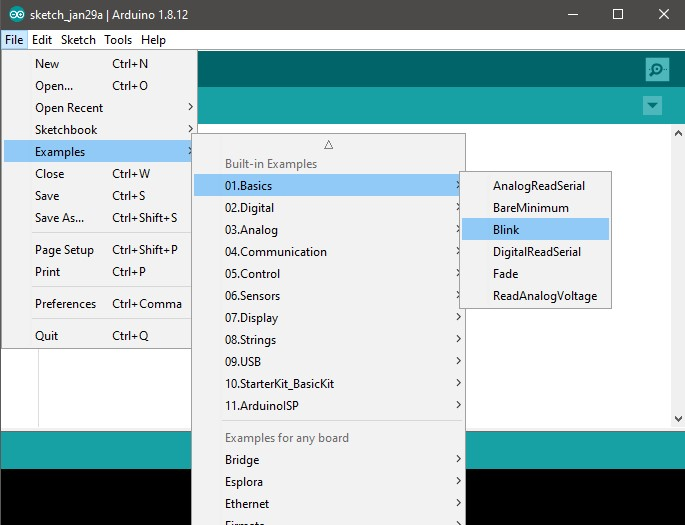
\includegraphics[width=0.8\textwidth]{arduino_ide_blink_example.jpg}
    \label{fig:ide-blink}
    \caption{Arduino IDE Example Code}
\end{figure}

The simplest Arduino example is the Blink code, which turns on and off an onboard LED.

\begin{lstlisting}
void setup() {
  // initialize digital pin LED_BUILTIN as an output.
  pinMode(LED_BUILTIN, OUTPUT);
}

// the loop function runs over and over again forever
void loop() {
  // turn the LED on (HIGH is the voltage level)
  digitalWrite(LED_BUILTIN, HIGH); 

  delay(1000);      // wait for a second

  // turn the LED off by making the voltage LOW
  digitalWrite(LED_BUILTIN, LOW);  
  
  delay(1000);      // wait for a second
}
\end{lstlisting}


There are a few common aspects present in the code of nearly every Arduino project, no matter how simple or complicated. \\


\lstinline[]!pinMode(<pin number>, <mode>)! sets a digital pin on the Arduino to be either an \lstinline[]!INPUT! or and \lstinline[]!OUTPUT!. \\


\lstinline[]!digitalWrite()! is used to set digital pins \lstinline[]!HIGH! and \lstinline[]!LOW!.



\pagebreak

Thinking back to the H-Bridge, to control the direction of the motor we want to control which switches are closed and which are open. Switches are generally active low - which means that they are off by default. To turn them on, in other words close them, we want to set pins to high. \\

To make it easier on ourselves, let's assign the pin numbers for each switch to a variable. Let's put these at the very top of our script, so that every function we write later can access the variables. 

\begin{lstlisting}
//Motor A
const int motorPin1  = 6;  // Pin 14 of L293
const int motorPin2  = 5;  // Pin 10 of L293
//Motor B
const int motorPin3  = 9; // Pin  7 of L293
const int motorPin4  = 8;  // Pin  2 of L293
\end{lstlisting}

The keyword \lstinline[]!const! means that the pin number cannot be changed. 
The value of the variables can be changed to any digital pin number on the Arduino, though make sure that the variable number matches the physical pin used. \\


Next we need to set the pin mode of the pins we're using, all the pin's for the motor need to be set to \lstinline[]!OUTPUT!.

\begin{lstlisting}
void setup(){
    //Set pins as outputs
    pinMode(motorPin1, OUTPUT);
    pinMode(motorPin2, OUTPUT);
    pinMode(motorPin3, OUTPUT);
    pinMode(motorPin4, OUTPUT);
}
\end{lstlisting}



\end{document}